\title{Results}

results...

\section{Validate}

Validate

\section{eSTATISTIK}

\subsection{Integration}

A number of general  issues presented themselves in the process of integrating the proof of concept from \citep{GIT:2015} into eSTATISTK design and production enviromment. Some of them are rather trivial, and practically all stem from limitations or particular properties of the eSTATISTIK tools.



 

\subsection{Implementation}

\subsection{Validation}

\section{Comparative View}

Comparative View

\begin{figure}
\centering
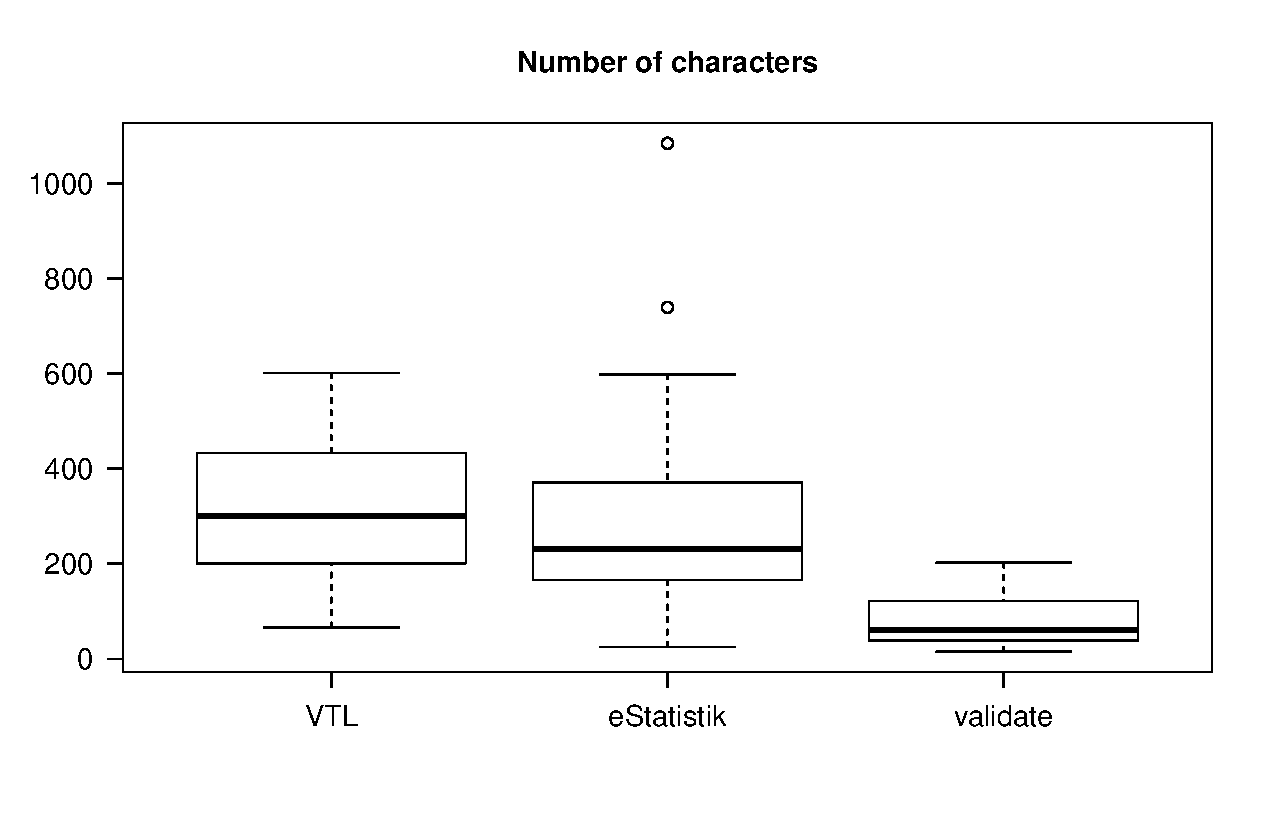
\includegraphics[width=0.9\textwidth]{fig/boxplot.pdf}
\caption{From left to right, the number of characters necessary
to specify the 18 rules in \code{VTL}, \code{eStatistik}, and \code{validate}.
Comment sections, empty lines and spurious whitespaces have been removed before
counting. }
\end{figure}

\begin{figure}
\centering
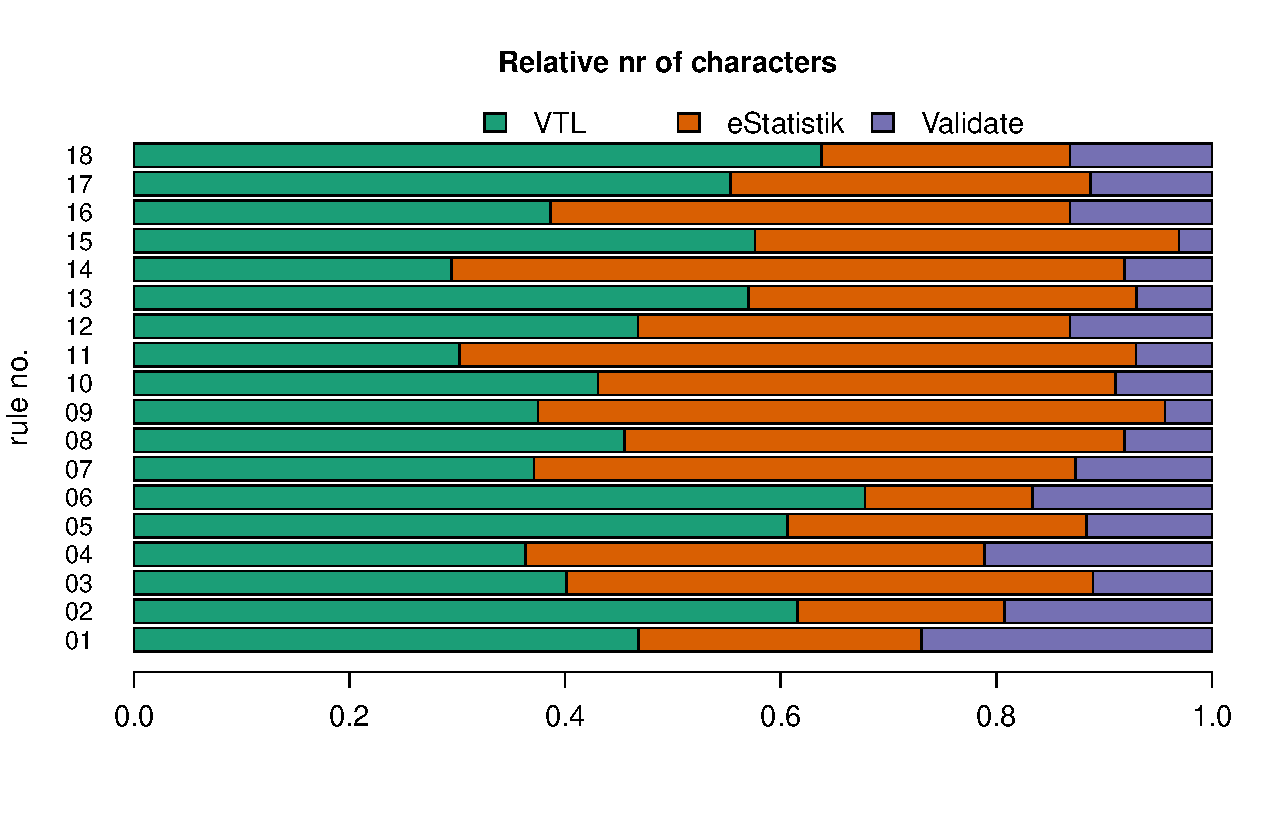
\includegraphics[width=0.9\textwidth]{fig/barplot.pdf}
\caption{The relative number of characters used by \code{VTL},
\code{eStatistik}, and \code{validate} to specify each of the 18 test rules.
Comment sections, empty lines and spurious white spaces have been removed
before counting. }
\end{figure}


\section{Summary}

Summary
